\documentclass[aspectratio=169]{beamer}
\usepackage{graphicx}
\usepackage{hyperref}
\usetheme{metropolis}
\title{Goals, Expectations, and Consequences}
\institute{Engineers for Exploration, UC San Diego}
\logo{
\includegraphics[height=.65cm,keepaspectratio]{e4e_logo_350x136.png}}
\setbeamertemplate{caption}[numbered]
\begin{document}
\maketitle
\begin{frame}
    What are goals, expectations, and consequences?
\end{frame}
\note[itemize]{
    \item Goals - desired results that team commits to within a specific timeframe
    \item Expectations - desired behaviors and values of the team/group
    \item Consequences - result of something occurring earlier
    \item Have students provide examples to demonstrate understanding
}
\begin{frame}
    What makes a good goal?
\end{frame}
\begin{frame}{SMART Goals}
    \begin{itemize}
        \item Specific - is concrete and tangible
        \item Measurable - has an objective measure of success
        \item Attainable - is challenging but achievable with available resources
        \item Relevant - meaningfully contributes to larger objectives
        \item Timely - has a deadline or timeline of progress
    \end{itemize}
\end{frame}
\note[itemize]{
    \item Specific - is concrete and tangible
    \item Measurable - has an objective measure of success
    \item Attainable - is challenging but achievable with available resources
    \item Relevant - meaningfully contributes to larger objectives
    \item Timely - has a deadline or timeline of progress
    \item Have students provide examples to demonstrate understanding
}
\begin{frame}
    What are the goals in your teams?
\end{frame}
\begin{frame}
    \centering
    What makes for good expectations?

    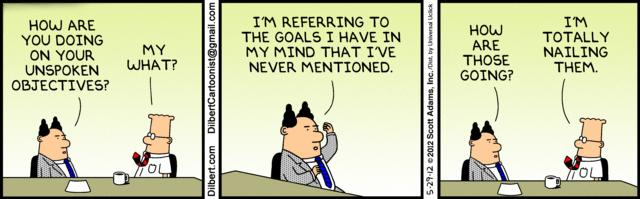
\includegraphics[width=0.8\textwidth,height=0.6\textheight,keepaspectratio]{dilbert-setting-expectations.jpg}
\end{frame}
\note[itemize]{
    \item Clear, Realistic, Consistent, Collaborative, Scoped
}
\begin{frame}
    \centering
    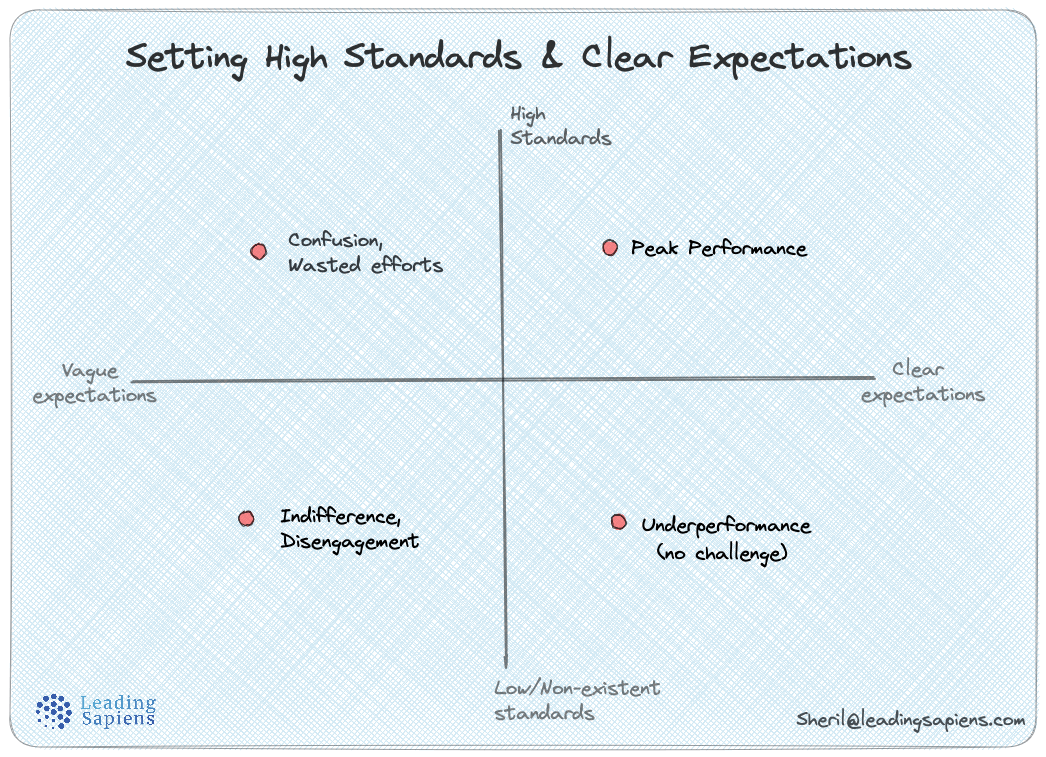
\includegraphics[width=\textwidth,height=0.8\textheight,keepaspectratio]{expectations_standards.png}
\end{frame}
\begin{frame}
    What are your expectations of your teams?
\end{frame}
\begin{frame}
    What makes for good consequences?
\end{frame}
\begin{frame}
    \begin{itemize}
        \item Directly linked
        \item Realistic
        \item Respectful
        \item Empowering
        \item Deliverable
    \end{itemize}
\end{frame}
\note[itemize]{
    \item Directly linked - should be linked directly to the action
    \item Realistic - ought to be realistic and achievable
    \item Respectful - should protect and promote the dignity of the person
    \item Empowering - should inspire and motivate the person to alter their behavior and enhance advancement
    \item Deliverable - should be known and agreeable to both parties with deliverable time limits
    \item These should be both positive and corrective consequences
    \item Remember back to our discussion on a just culture - where possible, ensure that people learn, and don't just focus on punitive punishment
}
\begin{frame}
    What consequences have you established in your team?
\end{frame}
\begin{frame}
    How can we ensure good communication of goals, expectations, and consequences?
\end{frame}
\end{document}
